\chapter{Oscillations and Waves}

\textbf{Periodic Motion} is a motion that regularly returns a certain position after fixed time.
\textbf{Simple Harmonic Motion} is a special kind of periodic motion where the magnitude of the 
net force acting on an object is proportional to the position of said object and its direction
opposite of the displacement of said object relative to its equilibrium position.

\section{Motion of an Object Attached to a Spring}

Consider the following system.

\begin{center}
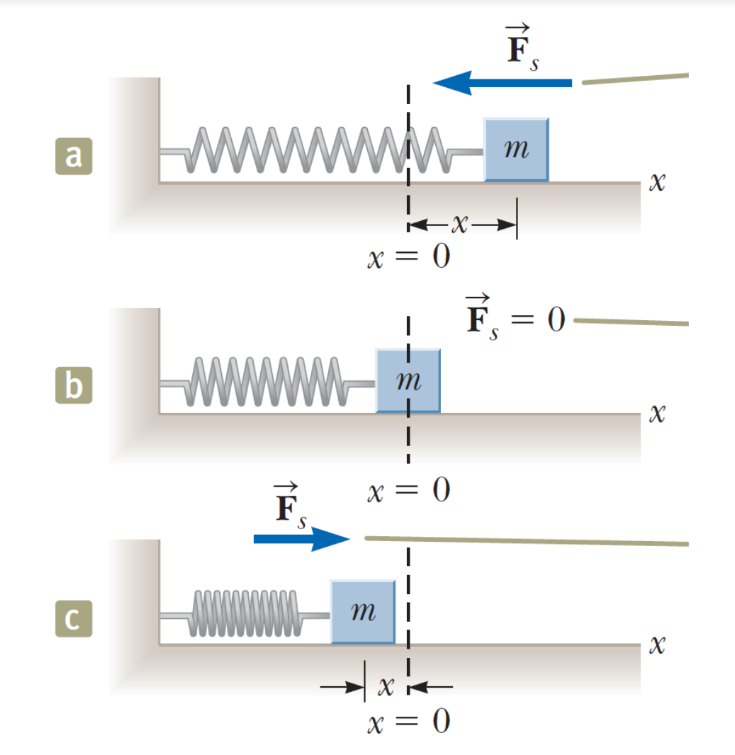
\includegraphics[scale=0.5]{oaw/spring01.png}\label{fig15.1}
\end{center}

When the spring is neither stretched or compressed, the block is at the \textbf{equilibirum position},
denoting as $x = 0$. When force is applied, the position of the block will move back and forth in an 
oscillating motion. We can model this using Hooke's law.

\begin{equation}\label{15.1}
    F_s = -kx
\end{equation} 

Here, we call $F_s$ the \textbf{restoring force} as it is always directed towards the equilibrium position.
Thus, it will always be opposite of the displacement of the block. Since there is some net force
acting on the object, even when released, we can apply Newton's second law of motion onto~\eqref{15.1}
to obtain

\begin{equation*}
    \sum F_x = ma_x \rightarrow -kx = ma_x
\end{equation*}

\begin{equation}\label{15.2}
    a_x = - \frac{k}{m}x
\end{equation}

This shows that the force applied on the object is proportional to $x$ and direction is opposite 
of the displacement. This is an example of a simple harmonic motion.

An example of how an object moves $-$ given the object starts at displacement $x=A$ and $x=0$ is the
equilibrium position:
\begin{itemize}
    \item Once released from rest, initial acceleration $a_i = -kA/m$ and speed is 0
    \item Once block is at $x=0$, acceleration is also zero and speed is at maximum
    \item Passing $x=0$, it moves with positive acceleration until $x=-A$, $a = +kA/m$, and speed is 0
    \item Moves back and passes $x=0$ again with maximum speed
\end{itemize}

In conclusion, the object oscillates between $x \in [-A, A]$. Note that we are consider this system
in the absence of friction. However, real-world systems are not frictionless, so please do keep that in mind.

\section{Analysis Model: Particle in Simple Harmonic Motion}

Recall equation from~\eqref{15.2}, we can turn $a$ into $d^2x / dt^2$ since accerelation is just
the second derivative of displacement and express it as
\begin{equation}\label{15.3}
    \frac{d^2x}{dt^2} = -\frac{k}{m}x
\end{equation}

We can then express $k/m$ as $\omega^2$ then rewrite~\eqref{15.3} as 
\begin{equation}\label{15.5}
    \frac{d^2x}{dt^2} = - \omega^2 x
\end{equation}

We now arrive at a differential equation that we need to solve. In essence, we are trying to 
find a function $x$ whose second-order derivative is the same as the original with a negative sign
and multiplied by $\omega^2$.
We have a few choices: polynomic with negative power, exponential, logarithmic, and trigonometric
functions. Our choice? \textit{Trigonometric functions}, specifically $\sin$ and $\cos$. Finally,
we have found a suitable function $x$.
\begin{equation}\label{15.6}
    x(t) = A\sin(\omega t + \phi)
\end{equation} 
where $A$, $\omega$, and $\phi$ are constant parameters of the motion. Then, we can plot $x$ as
a function of $t$. These parameters (and some more) will then represent the following:
\begin{itemize}
    \item $A$ represents the \textbf{amplitude} $-$ the maximum value of position such that $|x|\leq A$
    \item $\omega$ represents the \textbf{angular frequency} $-$ measure of how rapidly the oscillations
        are occurring, where \begin{equation}\label{15.9}
            \omega = \sqrt{\frac{k}{m}}
        \end{equation}
    \item $\phi$ represents the \textbf{phase constant} or \textbf{initial phase angle} $-$
        determined by the position and velocity position and velocity of object at $t=0$, where
        if $x=A$ at $t=0$, $\phi = 0$
\end{itemize}

Another quantity to know is $(\omega t + \phi)$ or the \textbf{phase} of the motion.
Notice that the value of $x(t)$ has the same value when the $\omega t$ increases by $2\pi$ radians.

Now, we will also introduce another value $T$ representing the \textbf{period} which refers to 
the time interval for an object to go through a full cycle of motion. This essentially means that 
the speed and position of the object at time $t$ and $t+T$ will be the same. This can be further
summarized $-$ using the property of phase $-$ down to 
\[ \left[\omega(t + T) + \phi\right] - (\omega t +\phi) = 2\pi \]
since when the phase is added by $2\pi$, the $x(t)$ reverts to its original value.

Simplifying the above equation gives us
\begin{equation}\label{15.10}
    T = \frac{2\pi}{\omega}
\end{equation}

One more quantity we should know is the \textbf{frequency} $f$, the inverse of the period.
Since the period is the time interval per oscillation, the frequency is oscillations per time interval.
This can be modeled under
\begin{equation}\label{15.11}
    f = \frac{1}{T} = \frac{\omega}{2\pi}
\end{equation}
and its units are cycles per second or \textit{hertz} (Hz). Rearranging the above equation yields
\begin{equation}\label{15.12}
    \omega = 2\pi f = \frac{2\pi}{T}
\end{equation}

If we converted $\omega$ back to its original value of $\sqrt{k/m}$, we will notice that $T$ and $f$
depend solely on the mass of the object and the force constant of the spring.

Additionally, since $x(t) = A\sin(\omega t + \phi)$ represents the position of the object, we can
find the velocity and acceleration squared of the object under S.H.M. using
\begin{eqnarray}
    v = \frac{dx}{dt} = \omega A\cos(\omega t + \phi)\label{15.15}\\
    a = \frac{d^2x}{dt^2} = -\omega^2 A\sin(\omega t + \phi)\label{15.16}
\end{eqnarray}

Notice from both equations that since $\cos$ and $\sin$ both have range of $[-1, 1]$, the range of 
the velocity and acceleration are as following
\begin{eqnarray}
    v_{\max} = \omega A\\
    a_{\max} = \omega^2 A
\end{eqnarray}

\section{Energy of Simple Harmonic Oscillator}

Once we have analyzed a S.H.M. with its forces, we now analyze it with its energy. Consider the 
same system from~\ref{fig15.1}. Let us make a few assumptions: that our spring has no mass and the 
surface is frictionless.

Recall equation~\eqref{15.15}, we can use it to express the kinetic energy of the block as 
\begin{equation}\label{15.19}
    K = \frac{1}{2}mv^2 = \frac{1}{2}m\left(\omega^2 A^2 \cos^2(\omega t + \phi)\right)
\end{equation}
We refer to this as the \textit{kinetic energy of a simple harmonic oscillator}.

Then, we can use equation~\eqref{15.16} for the elastic potential energy from the spring
\begin{equation}\label{15.20}
    U = \frac{1}{2}kx^2 = \frac{1}{2}k\left(A^2 \sin^2(\omega t + \phi)\right)
\end{equation}
We refer to this as the \textit{potential energy of a simple harmonic oscillator}.

\begin{center}\label{fig15.9}
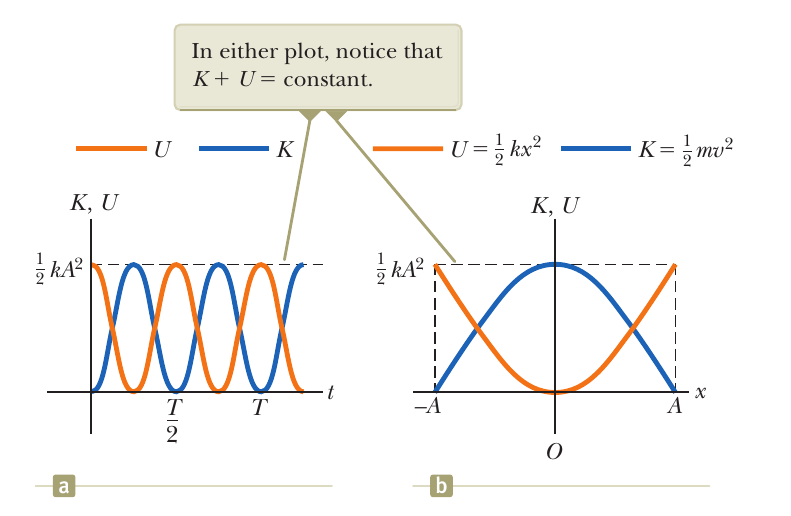
\includegraphics[scale=0.5]{images/oaw/fig15_9.png}
\end{center}
Once plotted, notice that $K$ and $U$ are always positive or zero. We can then express the total
mechanical energy of the system as 
\begin{equation}\label{fullE}
    E = K + U = \frac{1}{2}kA^2\left[ \cos^2(\omega t + \phi) + \sin^2(\omega t + \phi) \right]
\end{equation}

Using trigonometric identity, we can simplify $E$ down to 
\begin{equation}\label{15.21}
    E = \frac{1}{2}kA^2
\end{equation}

This shows that $E$ is a constant of the motion and proportional to the square of the amplitude.
Notice that at the end of the day, it is simply a conversion between the the kinetic and potential
energy. Thus, their sum will always be equal to $(1/2)kA^2$.

\section{Pendulum}

\begin{center}
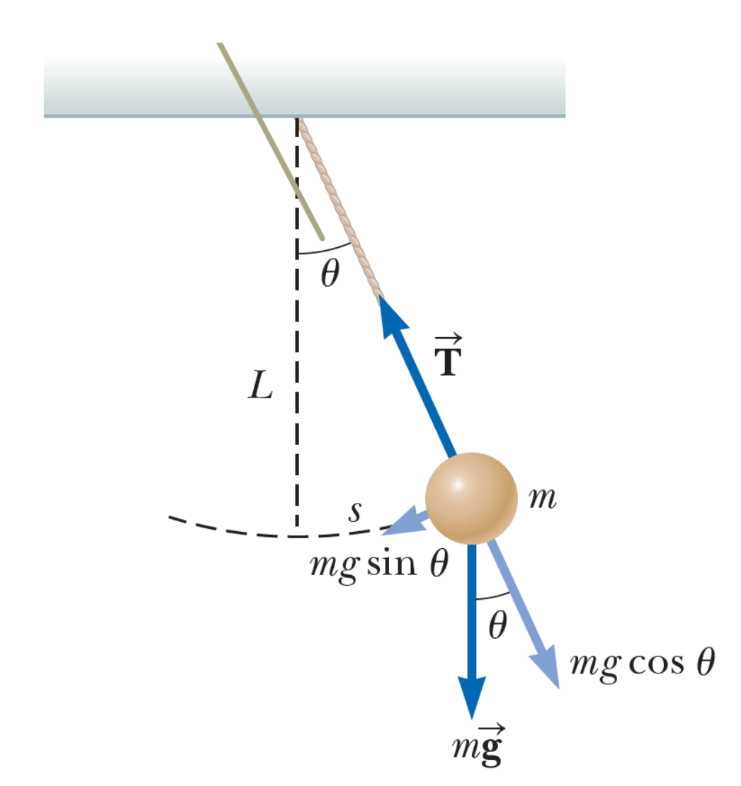
\includegraphics[scale=0.3]{images/oaw/pendulum01.png}
\end{center}

In order to analyze the motion of the pendulum, we can break down said motion into the vertical and
horizontal components. We can say that the tension $T = mg\cos\theta$ then completely ignore the motion's
vertical component as they cancel out. Therefore, the only remaining forces will be
\[\sum F_t = ma_t \implies -mg\sin\theta = m\frac{d^2s}{dt^2}\]
where $s$ is the tangential distance (displacement in circular motion). Once we cancel everything
and rearrange it such that it looks like our previous differential equation, we will get
\[ \frac{d^2s}{dt^2} = -g\sin\theta \]

This is where we need to face the harshness of reality. We cannot solve this equation, not without
a computer. However, we can use some approximation tricks to help us.

If the angle $\theta$ of swing is small, $\sin\theta \approx \theta$. We can also change $s$ into 
something easier to deal with. Since we know that $\theta = s/L$ where $L$ is the radius, we can
express $s$ as $\theta L$. With some manipulation, our equation then becomes
\[ \frac{d^2(\theta)}{dt^2} \approx -\frac{g}{L}\theta \]

Therefore, the (approximate) solution to this equation of motion is
\[ \theta(t) = A\sin(\omega t + \delta), \omega = \sqrt{\frac{g}{L}} \]

In this case, mass does not even matter to the oscillation. The only things that matter are the 
gravitational accerelation ($g$) and the length of the string attached to your pendulum ($L$).
Interestingly, this was how people made clocks back in the day.

\subsection{Equation of Motion on Rotation}

\begin{center}
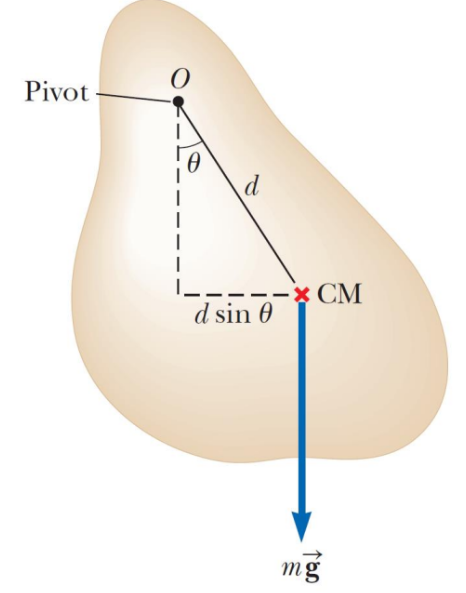
\includegraphics[scale=0.5]{images/oaw/rotation01.png}
\end{center}

Instead of Newton's equation, we now use $\vec{\tau} = I\vec{\alpha} = \vec{r}\times\vec{F}$.
From the diagram, we can see that the only thing generating torque is $m\vec{g}$. Let $r$ be the
distance from the pivot to the force (note that this distance is measured from $O$ to the point
perpendicular to the force), $r = d\sin\theta$. Now, torque will become $dmg\sin\theta$. Since
the torque is going clock-wise, the sign is negative. With some manipulation, our final 
approximate solution becomes
\[ \frac{d^2\theta}{dt^2} \approx -\frac{mgd}{I}\theta \]

Again, we can see that this is another simple harmonic motion where $\omega = \sqrt{(mgd)/I}$.

\subsection{Energy of Simple Harmonic Oscillator}

We can first find the kinetic and potential energy by
\begin{align*}
    K &= \frac{1}{2}mv^2 = \frac{1}{2}m\omega^2A^2\sin^2(\omega t + \phi)\\
    U &= \frac{1}{2}kx^2 = \frac{1}{2}A^2\cos^2(\omega t + \phi)
\end{align*}

Then, we can derive the total energy by
\begin{align*}
    E &= K + U\\
    &= \frac{1}{2}m\omega^2A^2\sin^2(\omega t + \phi) + \frac{1}{2}A^2\cos^2(\omega t + \phi)\\
    &= \frac{1}{2}kA^2 ( \sin^2(\omega t + phi) + \cos^2(\omega t + phi))\\
    &= \frac{1}{2}kA^2
\end{align*}
Note that since $\omega^2 \ k / m$, $(1/2)m(k/m) = (1/2)k$.

What does this mean? At any moment in time, the sum of the energy of the system must remain the same.
This aligns with the conservation of energy.